\documentclass[11pt]{report}

% Paquetes y configuraciones adicionales
\usepackage{graphicx}
\usepackage[export]{adjustbox}
\usepackage{caption}
\usepackage{float}
\usepackage{titlesec}
\usepackage{geometry}
\usepackage[hidelinks]{hyperref}
\usepackage{titling}
\usepackage{titlesec}
\usepackage{parskip}
\usepackage{wasysym}
\usepackage{tikzsymbols}
\usepackage{fancyvrb}
\usepackage{xurl}
\usepackage{hyperref}
\usepackage{subcaption}

\usepackage{listings}
\usepackage{xcolor}

\usepackage[spanish]{babel}

\newcommand{\subtitle}[1]{
  \posttitle{
    \par\end{center}
    \begin{center}\large#1\end{center}
    \vskip0.5em}
}

% Configura los márgenes
\geometry{
  left=2cm,   % Ajusta este valor al margen izquierdo deseado
  right=2cm,  % Ajusta este valor al margen derecho deseado
  top=3cm,
  bottom=3cm,
}

% Configuración de los títulos de las secciones
\titlespacing{\section}{0pt}{\parskip}{\parskip}
\titlespacing{\subsection}{0pt}{\parskip}{\parskip}
\titlespacing{\subsubsection}{0pt}{\parskip}{\parskip}

% Redefinir el formato de los capítulos y añadir un punto después del número
\makeatletter
\renewcommand{\@makechapterhead}[1]{%
  \vspace*{0\p@} % Ajusta este valor para el espaciado deseado antes del título del capítulo
  {\parindent \z@ \raggedright \normalfont
    \ifnum \c@secnumdepth >\m@ne
        \huge\bfseries \thechapter.\ % Añade un punto después del número
    \fi
    \interlinepenalty\@M
    #1\par\nobreak
    \vspace{10pt} % Ajusta este valor para el espacio deseado después del título del capítulo
  }}
\makeatother

% Configura para que cada \chapter no comience en una pagina nueva
\makeatletter
\renewcommand\chapter{\@startsection{chapter}{0}{\z@}%
    {-3.5ex \@plus -1ex \@minus -.2ex}%
    {2.3ex \@plus.2ex}%
    {\normalfont\Large\bfseries}}
\makeatother

% Configurar los colores para el código
\definecolor{codegreen}{rgb}{0,0.6,0}
\definecolor{codegray}{rgb}{0.5,0.5,0.5}
\definecolor{codepurple}{rgb}{0.58,0,0.82}
\definecolor{backcolour}{rgb}{0.95,0.95,0.92}

% Configurar el estilo para el código
\lstdefinestyle{mystyle}{
  backgroundcolor=\color{backcolour},   
  commentstyle=\color{codegreen},
  keywordstyle=\color{magenta},
  numberstyle=\tiny\color{codegray},
  stringstyle=\color{codepurple},
  basicstyle=\ttfamily\footnotesize,
  breakatwhitespace=false,         
  breaklines=true,                 
  captionpos=b,                    
  keepspaces=true,                 
  numbers=left,                    
  numbersep=5pt,                  
  showspaces=false,                
  showstringspaces=false,
  showtabs=false,                  
  tabsize=2
}

\begin{document}

% Portada del informe
\title{Practica 02. Análisis de la Base de Datos de Gestión Docente}
\subtitle{Bases de Datos}
\author{Cheuk Kelly Ng Pante (alu0101364544@ull.edu.es)}
\date{\today}

\maketitle

\pagestyle{empty} % Desactiva la numeración de página para el índice

% Índice
\tableofcontents

% Nueva página
\cleardoublepage

\pagestyle{plain} % Vuelve a activar la numeración de página
\setcounter{page}{1} % Reinicia el contador de página a 1

% Secciones del informe
% Capitulo 1
\chapter{Comprender el significado de los atributos y el sentido de las relaciones expresadas en las tablas}
\begin{itemize}
  \item \textbf{Departamento:} Tabla que contiene información sobre los departamentos, tanto el código de cada uno, como el nombre.
  \item \textbf{Área:} La clave primaria es CAR (código de área). Cada área pertenece a un único departamento, de ahí la relación.
  \item \textbf{Profesor:} DNI es la clave primaria. Tiene en común con la tabla anterior el código de área (CAR).
  \item \textbf{Asignatura:} Una asignatura sólo puede pertenecer a un área, la clave primaria es CAS (código de asignatura), que es el identificador de la asignatura.
  \item \textbf{Plan\_Docente:} En esta tabla se refleja las asignaciones de los profesores a las asignaturas, y su relación entre ellos. También se ven los periodos en los que se han impartido las asignaturas.
\end{itemize}

% Capitulo 2
\chapter{Enumerar y justificar las implicaciones derivadas de las definiciones de claves primarias y ajenas realizadas en el diseño.}
La clave primaria es el primer índice de búsqueda para localizar registros únicos, su principal característica es que es un índice único.

% Capitulo 3
\chapter{Representar el diagrama de jerarquía referencial de este diseño y especificar un posible orden de creación/borrado de objetos.}
\begin{figure}[H]
  \centering
  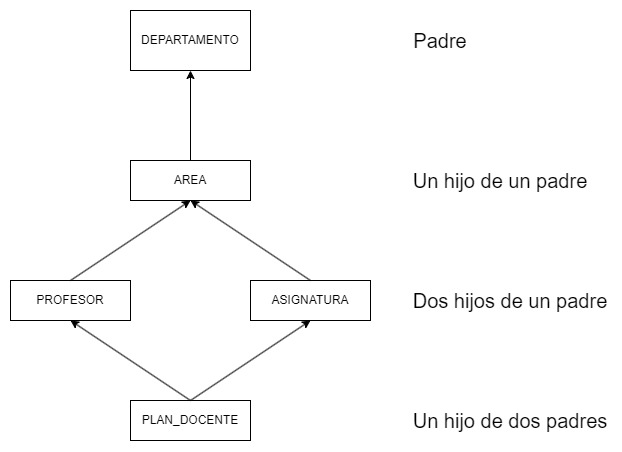
\includegraphics[width=0.63\textwidth]{img/diagrama_jerarquia.jpg}
  \caption{Diagrama de jerarquía referencial}
\end{figure}

% Capitulo 4
\chapter{Describir posibles políticas de mantenimiento de la integridad referencial para esta base de datos.}
Existen niveles de borrado, cuando se borre algún atributo en departamento, si este tiene que ver con otras tablas, se irá borrando en las demás tablas en
cascada. Esto pasará siempre que se borre desde una tabla un atributo que se relaciones con otras, a no ser que sea de nivel inferior.

% Capitulo 5
\chapter{Representar gráficamente el esquema conceptual de la base de datos utilizando el modelo E/R.}
\begin{figure}[H]
  \centering
  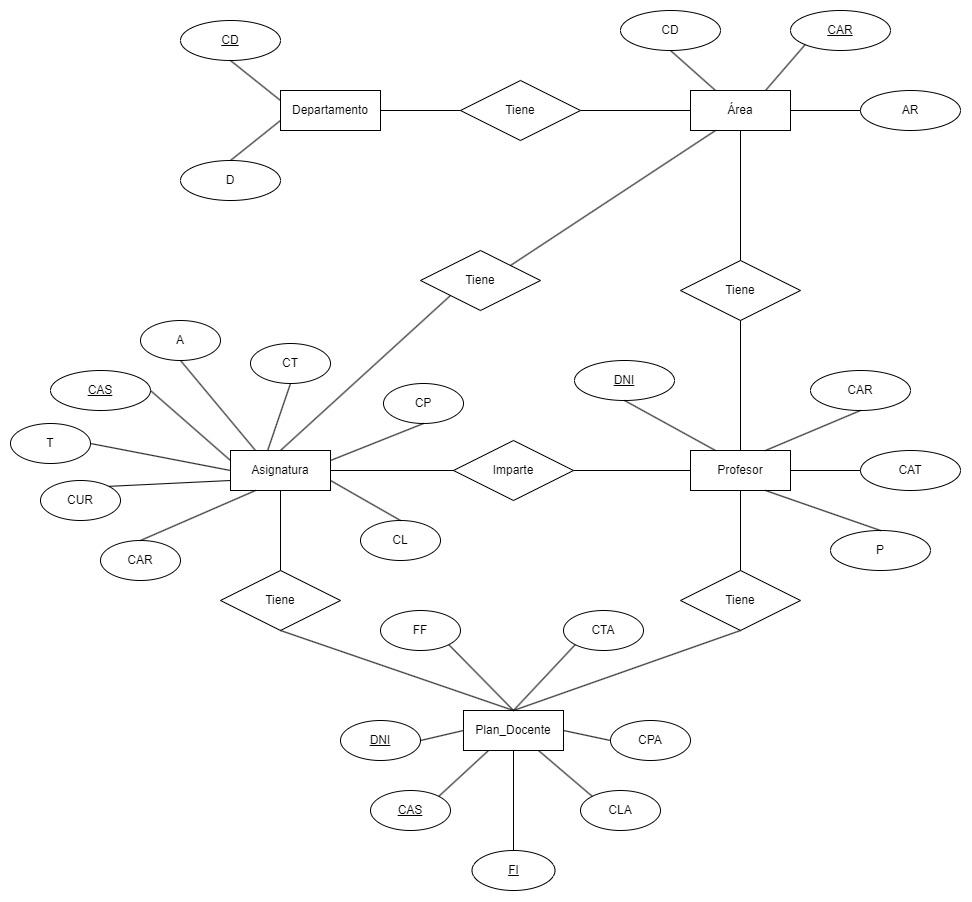
\includegraphics[width=0.68\textwidth]{img/modelo_E-R_P2.jpg}
  \caption{Esquema Entidad Relacion}
\end{figure}

% Capitulo 6
\chapter{Enuncia y justifica diferentes condiciones de integridad generales que, a tu juicio, deben satisfacerse en esta base de datos}
\begin{itemize}
  \item \textbf{FI \textless{} FF:} Ya que la fecha de inicio tiene que ser menor que la de final, para que estos campos tengan sentido.
  \item \textbf{CTA $\leq$ CT:} Un profesor no tiene porqué tener asignados todos los créditos de una asignatura. (Lo mismo con CPA y CLA)
\end{itemize}

\end{document}